
\section{Diode I}
\label{section:diode_1}
\begin{frame}%STARTCONTENT

\frametitle{Anwendung}
\begin{columns}
    \begin{column}{0.48\textwidth}
    \begin{itemize}
  \item Eine Diode lässt den Stromfluss nur in eine Richtung durch
  \item In die andere Richtung wirkt sie wie ein hoher Widerstand
  \item Dioden werden u.a. zur Gleichrichtung von Wechselspannung eingesetzt
  \end{itemize}

    \end{column}
   \begin{column}{0.48\textwidth}
       
\begin{figure}
    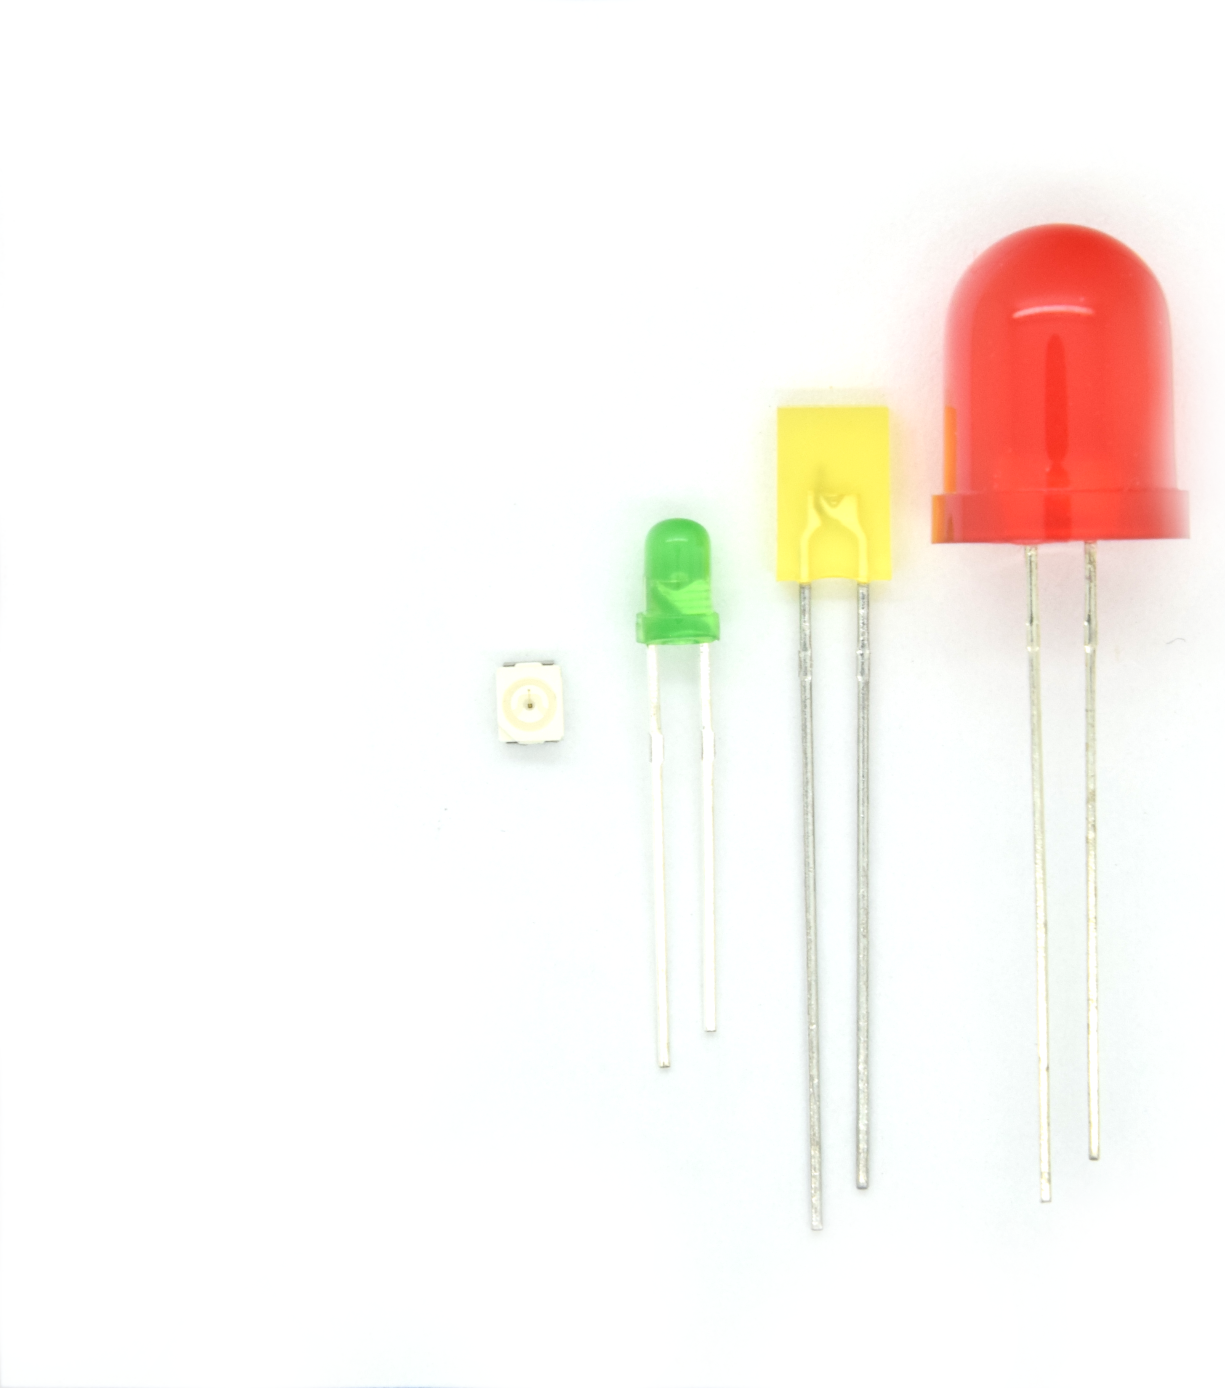
\includegraphics[width=0.85\textwidth]{foto/6}
    \caption{\scriptsize Diverse LED in verschiedenen Bauformen und Farben}
    \label{e_led}
\end{figure}

   \end{column}
\end{columns}

\end{frame}

\begin{frame}
\only<1>{
\begin{QQuestion}{EC501}{Eine in Sperrrichtung betriebene Diode zeichnet sich insbesondere aus durch~...}{eine hohe Induktivität.}
{eine hohe Kapazität.}
{eine geringe Impedanz.}
{einen hohen Widerstand.}
\end{QQuestion}

}
\only<2>{
\begin{QQuestion}{EC501}{Eine in Sperrrichtung betriebene Diode zeichnet sich insbesondere aus durch~...}{eine hohe Induktivität.}
{eine hohe Kapazität.}
{eine geringe Impedanz.}
{\textbf{\textcolor{DARCgreen}{einen hohen Widerstand.}}}
\end{QQuestion}

}
\end{frame}

\begin{frame}
\only<1>{
\begin{QQuestion}{EC502}{Wofür können Halbleiterdioden beispielsweise verwendet werden?}{zur Speicherung von Wechselströmen}
{zur Gleichrichtung von Wechselspannung}
{als Widerstand in Netzteilen}
{als Verstärker in Stromversorgungen}
\end{QQuestion}

}
\only<2>{
\begin{QQuestion}{EC502}{Wofür können Halbleiterdioden beispielsweise verwendet werden?}{zur Speicherung von Wechselströmen}
{\textbf{\textcolor{DARCgreen}{zur Gleichrichtung von Wechselspannung}}}
{als Widerstand in Netzteilen}
{als Verstärker in Stromversorgungen}
\end{QQuestion}

}
\end{frame}

\begin{frame}
\frametitle{Schwellenspannung}
\begin{columns}
    \begin{column}{0.48\textwidth}
    \begin{itemize}
  \item Damit eine Diode in Durchlassrichtung leitet, muss eine bestimmte Spannung -- die Schwellenspannung oder Durchlassspannung -- überschritten werden
  \item Je nach Basis des chemischen Elements ist die Schwellenspannung unterschiedlich hoch
  \end{itemize}

    \end{column}
   \begin{column}{0.48\textwidth}
       \begin{itemize}
  \item Germanium: \qty{0,2}{\volt}-\qty{0,4}{\volt}
  \item Silizium: \qty{0,6}{\volt}-\qty{0,8}{\volt}
  \item LED (Rot): \qty{1,6}{\volt}-\qty{2,2}{\volt}
  \item LED (Gelb, Grün): \qty{1,9}{\volt}-\qty{2,5}{\volt}
  \item LED (Blau, Weiß): \qty{2,7}{\volt}-\qty{3,5}{\volt}
  \end{itemize}

   \end{column}
\end{columns}

\end{frame}

\begin{frame}
\only<1>{
\begin{QQuestion}{EC503}{Welche typischen Schwellspannungen haben Germanium- und Siliziumdioden? Sie liegen bei~...}{Germanium zwischen \qtyrange{0,6}{0,8}{\V}, bei Silizium \qtyrange{1,4}{1,6}{\V}.}
{Germanium zwischen \qtyrange{0,6}{0,8}{\V}, bei Silizium zwischen \qtyrange{0,2}{0,4}{\V}.}
{Germanium zwischen \qtyrange{1,4}{1,6}{\V}, bei Silizium \qtyrange{0,6}{0,8}{\V}.}
{Germanium zwischen \qtyrange{0,2}{0,4}{\V}, bei Silizium zwischen \qtyrange{0,6}{0,8}{\V}.}
\end{QQuestion}

}
\only<2>{
\begin{QQuestion}{EC503}{Welche typischen Schwellspannungen haben Germanium- und Siliziumdioden? Sie liegen bei~...}{Germanium zwischen \qtyrange{0,6}{0,8}{\V}, bei Silizium \qtyrange{1,4}{1,6}{\V}.}
{Germanium zwischen \qtyrange{0,6}{0,8}{\V}, bei Silizium zwischen \qtyrange{0,2}{0,4}{\V}.}
{Germanium zwischen \qtyrange{1,4}{1,6}{\V}, bei Silizium \qtyrange{0,6}{0,8}{\V}.}
{\textbf{\textcolor{DARCgreen}{Germanium zwischen \qtyrange{0,2}{0,4}{\V}, bei Silizium zwischen \qtyrange{0,6}{0,8}{\V}.}}}
\end{QQuestion}

}
\end{frame}

\begin{frame}
\frametitle{Schottky-Diode}
\begin{itemize}
  \item Erlaubt eine hohe Schaltfrequenz
  \item Nur eine sehr niedrige Schwellenspannung von \qty{0,4}{\volt} bis unter \qty{0,1}{\volt} ist nötig
  \end{itemize}
\end{frame}

\begin{frame}
\only<1>{
\begin{QQuestion}{EC504}{Welches sind die Haupteigenschaften einer Schottkydiode?}{Sehr niedrige Durchlassspannung und sehr hohe Schaltfrequenz.}
{Sehr niedrige Durchlassspannung und sehr niedrige Schaltfrequenz.}
{Sehr hohe Durchlassspannung und sehr hohe Schaltfrequenz.}
{Sehr hohe Durchlassspannung und sehr niedrige Schaltfrequenz.}
\end{QQuestion}

}
\only<2>{
\begin{QQuestion}{EC504}{Welches sind die Haupteigenschaften einer Schottkydiode?}{\textbf{\textcolor{DARCgreen}{Sehr niedrige Durchlassspannung und sehr hohe Schaltfrequenz.}}}
{Sehr niedrige Durchlassspannung und sehr niedrige Schaltfrequenz.}
{Sehr hohe Durchlassspannung und sehr hohe Schaltfrequenz.}
{Sehr hohe Durchlassspannung und sehr niedrige Schaltfrequenz.}
\end{QQuestion}

}
\end{frame}

\begin{frame}
\frametitle{Kennlinien}
\end{frame}

\begin{frame}
\only<1>{
\begin{PQuestion}{EC506}{Welche Diode wird durch Kennlinie 2 charakterisiert?}{Germaniumdiode}
{Siliziumdiode}
{Schottkydiode}
{Leuchtdiode}
{\DARCimage{1.0\linewidth}{307include}}\end{PQuestion}

}
\only<2>{
\begin{PQuestion}{EC506}{Welche Diode wird durch Kennlinie 2 charakterisiert?}{\textbf{\textcolor{DARCgreen}{Germaniumdiode}}}
{Siliziumdiode}
{Schottkydiode}
{Leuchtdiode}
{\DARCimage{1.0\linewidth}{307include}}\end{PQuestion}

}
\end{frame}

\begin{frame}
\only<1>{
\begin{PQuestion}{EC507}{Welche Diode wird durch Kennlinie 3 charakterisiert?}{Schottkydiode}
{Leuchtdiode}
{Siliziumdiode}
{Germaniumdiode}
{\DARCimage{1.0\linewidth}{307include}}\end{PQuestion}

}
\only<2>{
\begin{PQuestion}{EC507}{Welche Diode wird durch Kennlinie 3 charakterisiert?}{Schottkydiode}
{Leuchtdiode}
{\textbf{\textcolor{DARCgreen}{Siliziumdiode}}}
{Germaniumdiode}
{\DARCimage{1.0\linewidth}{307include}}\end{PQuestion}

}
\end{frame}

\begin{frame}
\only<1>{
\begin{PQuestion}{EC508}{Welche Diode wird durch Kennlinie 4 charakterisiert?}{Leuchtdiode}
{Siliziumdiode}
{Schottkydiode}
{Germaniumdiode}
{\DARCimage{1.0\linewidth}{307include}}\end{PQuestion}

}
\only<2>{
\begin{PQuestion}{EC508}{Welche Diode wird durch Kennlinie 4 charakterisiert?}{\textbf{\textcolor{DARCgreen}{Leuchtdiode}}}
{Siliziumdiode}
{Schottkydiode}
{Germaniumdiode}
{\DARCimage{1.0\linewidth}{307include}}\end{PQuestion}

}
\end{frame}

\begin{frame}
\only<1>{
\begin{PQuestion}{EC505}{Welche Diode wird durch Kennlinie 1 charakterisiert?}{Germaniumdiode}
{Siliziumdiode}
{Schottkydiode}
{Leuchtdiode}
{\DARCimage{1.0\linewidth}{307include}}\end{PQuestion}

}
\only<2>{
\begin{PQuestion}{EC505}{Welche Diode wird durch Kennlinie 1 charakterisiert?}{Germaniumdiode}
{Siliziumdiode}
{\textbf{\textcolor{DARCgreen}{Schottkydiode}}}
{Leuchtdiode}
{\DARCimage{1.0\linewidth}{307include}}\end{PQuestion}

}
\end{frame}

\begin{frame}
\frametitle{Leitende Diode}
\begin{columns}
    \begin{column}{0.48\textwidth}
    \begin{itemize}
  \item Eine Diode leitet immer dann, wenn die Spannung an der Anode um die Schwellenspannung positiver ist als an der Kathode
  \item Gilt auch für negative Spannungen
  \item In der Prüfung kommen nur Siliziumdioden mit \qty{0,7}{\volt} Schwellenspannung vor
  \end{itemize}

    \end{column}
   \begin{column}{0.48\textwidth}
       
\begin{figure}
    \DARCimage{0.85\linewidth}{113include}
    \caption{\scriptsize Spannungen an einer leitenden Siliziumdiode}
    \label{e_leitende_siliziumdiode}
\end{figure}


   \end{column}
\end{columns}

\end{frame}

\begin{frame}
\only<1>{
\begin{QQuestion}{EC513}{Bei welcher Bedingung wird eine Siliziumdiode leitend?}{An der Anode liegen \qty{5,7}{\V}, an der Kathode \qty{5,0}{\V} an.}
{An der Anode liegen \qty{5,7}{\V}, an der Kathode \qty{6,4}{\V} an.}
{An der Anode liegen \qty{5,0}{\V}, an der Kathode \qty{5,1}{\V} an.}
{An der Anode liegen \qty{5,0}{\V}, an der Kathode \qty{5,7}{\V} an.}
\end{QQuestion}

}
\only<2>{
\begin{QQuestion}{EC513}{Bei welcher Bedingung wird eine Siliziumdiode leitend?}{\textbf{\textcolor{DARCgreen}{An der Anode liegen \qty{5,7}{\V}, an der Kathode \qty{5,0}{\V} an.}}}
{An der Anode liegen \qty{5,7}{\V}, an der Kathode \qty{6,4}{\V} an.}
{An der Anode liegen \qty{5,0}{\V}, an der Kathode \qty{5,1}{\V} an.}
{An der Anode liegen \qty{5,0}{\V}, an der Kathode \qty{5,7}{\V} an.}
\end{QQuestion}

}
\end{frame}

\begin{frame}
\only<1>{
\begin{question2x2}{EC510}{Die Auswahlantworten enthalten Siliziumdioden mit unterschiedlichen Arbeitspunkten. Bei welcher Antwort befindet sich die Diode in leitendem Zustand?}{\DARCimage{1.0\linewidth}{110include}}
{\DARCimage{1.0\linewidth}{109include}}
{\DARCimage{1.0\linewidth}{111include}}
{\DARCimage{1.0\linewidth}{112include}}
\end{question2x2}

}
\only<2>{
\begin{question2x2}{EC510}{Die Auswahlantworten enthalten Siliziumdioden mit unterschiedlichen Arbeitspunkten. Bei welcher Antwort befindet sich die Diode in leitendem Zustand?}{\DARCimage{1.0\linewidth}{110include}}
{\textbf{\textcolor{DARCgreen}{\DARCimage{1.0\linewidth}{109include}}}}
{\DARCimage{1.0\linewidth}{111include}}
{\DARCimage{1.0\linewidth}{112include}}
\end{question2x2}

}
\end{frame}

\begin{frame}
\only<1>{
\begin{question2x2}{EC509}{Die Auswahlantworten enthalten Siliziumdioden mit unterschiedlichen Arbeitspunkten. Bei welcher Antwort befindet sich die Diode in leitendem Zustand?}{\DARCimage{1.0\linewidth}{116include}}
{\DARCimage{1.0\linewidth}{114include}}
{\DARCimage{1.0\linewidth}{115include}}
{\DARCimage{1.0\linewidth}{113include}}
\end{question2x2}

}
\only<2>{
\begin{question2x2}{EC509}{Die Auswahlantworten enthalten Siliziumdioden mit unterschiedlichen Arbeitspunkten. Bei welcher Antwort befindet sich die Diode in leitendem Zustand?}{\DARCimage{1.0\linewidth}{116include}}
{\DARCimage{1.0\linewidth}{114include}}
{\DARCimage{1.0\linewidth}{115include}}
{\textbf{\textcolor{DARCgreen}{\DARCimage{1.0\linewidth}{113include}}}}
\end{question2x2}

}
\end{frame}

\begin{frame}
\only<1>{
\begin{question2x2}{EC511}{Die Auswahlantworten enthalten Siliziumdioden mit unterschiedlichen Arbeitspunkten. Bei welcher Antwort befindet sich die Diode in leitendem Zustand?}{\DARCimage{1.0\linewidth}{118include}}
{\DARCimage{1.0\linewidth}{117include}}
{\DARCimage{1.0\linewidth}{119include}}
{\DARCimage{1.0\linewidth}{120include}}
\end{question2x2}

}
\only<2>{
\begin{question2x2}{EC511}{Die Auswahlantworten enthalten Siliziumdioden mit unterschiedlichen Arbeitspunkten. Bei welcher Antwort befindet sich die Diode in leitendem Zustand?}{\DARCimage{1.0\linewidth}{118include}}
{\textbf{\textcolor{DARCgreen}{\DARCimage{1.0\linewidth}{117include}}}}
{\DARCimage{1.0\linewidth}{119include}}
{\DARCimage{1.0\linewidth}{120include}}
\end{question2x2}

}
\end{frame}

\begin{frame}
\only<1>{
\begin{question2x2}{EC512}{Die Auswahlantworten enthalten Siliziumdioden mit unterschiedlichen Arbeitspunkten. Bei welcher Antwort befindet sich die Diode in leitendem Zustand?}{\DARCimage{1.0\linewidth}{121include}}
{\DARCimage{1.0\linewidth}{122include}}
{\DARCimage{1.0\linewidth}{123include}}
{\DARCimage{1.0\linewidth}{124include}}
\end{question2x2}

}
\only<2>{
\begin{question2x2}{EC512}{Die Auswahlantworten enthalten Siliziumdioden mit unterschiedlichen Arbeitspunkten. Bei welcher Antwort befindet sich die Diode in leitendem Zustand?}{\textbf{\textcolor{DARCgreen}{\DARCimage{1.0\linewidth}{121include}}}}
{\DARCimage{1.0\linewidth}{122include}}
{\DARCimage{1.0\linewidth}{123include}}
{\DARCimage{1.0\linewidth}{124include}}
\end{question2x2}

}
\end{frame}

\begin{frame}
\frametitle{LED Anwendung }
\begin{columns}
    \begin{column}{0.48\textwidth}
    \begin{itemize}
  \item Eine LED dient als Leuchtanzeige
  \end{itemize}

    \end{column}
   \begin{column}{0.48\textwidth}
       
\begin{figure}
    \DARCimage{0.85\linewidth}{324include}
    \caption{\scriptsize LED mit Vorwiderstand}
    \label{e_led_schaltung}
\end{figure}


   \end{column}
\end{columns}

\end{frame}

\begin{frame}
\only<1>{
\begin{PQuestion}{EC514}{Wozu dient die folgende Schaltung?}{Spannungserhöhung}
{Leuchtanzeige}
{Leistungsüberwachung}
{Stromgewinnung}
{\DARCimage{0.75\linewidth}{324include}}\end{PQuestion}

}
\only<2>{
\begin{PQuestion}{EC514}{Wozu dient die folgende Schaltung?}{Spannungserhöhung}
{\textbf{\textcolor{DARCgreen}{Leuchtanzeige}}}
{Leistungsüberwachung}
{Stromgewinnung}
{\DARCimage{0.75\linewidth}{324include}}\end{PQuestion}

}
\end{frame}

\begin{frame}
\frametitle{Vorwiderstand}
\begin{columns}
    \begin{column}{0.48\textwidth}
    \begin{itemize}
  \item Da die LED selbst kaum einen Widerstand hat, würde sie bei einem direkten Anschluss an eine Spannungsquelle wie ein Kurzschluss wirken
  \item Mit einem Vorwiderstand wird der Durchlassstrom begrenzt
  \end{itemize}

    \end{column}
   \begin{column}{0.48\textwidth}
       
\begin{figure}
    \DARCimage{0.85\linewidth}{324include}
    \caption{\scriptsize LED mit Vorwiderstand}
    \label{e_led_schaltung}
\end{figure}


   \end{column}
\end{columns}

\end{frame}

\begin{frame}\begin{itemize}
  \item Berechnung: $R = \dfrac{U_q -- U_{LED}}{I_D}$
  \item $U_q$: Spannungsquelle
  \item $U_{LED}$: Schwellenspannung LED
  \item $I_D$: Durchlassstrom
  \end{itemize}
\end{frame}

\begin{frame}
\only<1>{
\begin{QQuestion}{EC515}{Eine Leuchtdiode mit einer Durchlassspannung von \qty{1,4}{\V} und einem Durchlassstrom von \qty{20}{\mA} soll an eine Spannungsquelle von \qty{5,0}{\V} angeschlossen werden. Berechnen Sie den Vorwiderstand. Die Größe des benötigten Vorwiderstandes beträgt~...}{\qty{180}{\ohm}.}
{\qty{250}{\ohm}.}
{\qty{70}{\ohm}.}
{\qty{320}{\ohm}.}
\end{QQuestion}

}
\only<2>{
\begin{QQuestion}{EC515}{Eine Leuchtdiode mit einer Durchlassspannung von \qty{1,4}{\V} und einem Durchlassstrom von \qty{20}{\mA} soll an eine Spannungsquelle von \qty{5,0}{\V} angeschlossen werden. Berechnen Sie den Vorwiderstand. Die Größe des benötigten Vorwiderstandes beträgt~...}{\textbf{\textcolor{DARCgreen}{\qty{180}{\ohm}.}}}
{\qty{250}{\ohm}.}
{\qty{70}{\ohm}.}
{\qty{320}{\ohm}.}
\end{QQuestion}

}
\end{frame}

\begin{frame}
\only<1>{
\begin{PQuestion}{EC516}{Folgende Schaltung einer Leuchtdiode wird an einer Betriebsspannung von \qty{5,5}{\V} betrieben. Der Strom durch die Leuchtdiode soll \qty{25}{\mA} betragen, wobei die Durchlassspannung \qty{1,75}{\V} beträgt. Der notwendige Vorwiderstand muss folgende Werte haben:}{\qty{150}{\ohm}/\qty{0,1}{\W}}
{\qty{150}{\ohm}/\qty{0,06}{\W}}
{\qty{70}{\ohm}/\qty{0,1}{\W}}
{\qty{70}{\ohm}/\qty{0,06}{\W}}
{\DARCimage{0.75\linewidth}{324include}}\end{PQuestion}

}
\only<2>{
\begin{PQuestion}{EC516}{Folgende Schaltung einer Leuchtdiode wird an einer Betriebsspannung von \qty{5,5}{\V} betrieben. Der Strom durch die Leuchtdiode soll \qty{25}{\mA} betragen, wobei die Durchlassspannung \qty{1,75}{\V} beträgt. Der notwendige Vorwiderstand muss folgende Werte haben:}{\textbf{\textcolor{DARCgreen}{\qty{150}{\ohm}/\qty{0,1}{\W}}}}
{\qty{150}{\ohm}/\qty{0,06}{\W}}
{\qty{70}{\ohm}/\qty{0,1}{\W}}
{\qty{70}{\ohm}/\qty{0,06}{\W}}
{\DARCimage{0.75\linewidth}{324include}}\end{PQuestion}

}
\end{frame}

\begin{frame}
\frametitle{Z-Diode}
\begin{columns}
    \begin{column}{0.48\textwidth}
    \begin{itemize}
  \item Normalerweise liegt die maximale Sperrspannung einer Diode bei ca. \qty{1000}{\volt}
  \item Bei Z-Dioden erfolgt ein Spannungsdurchbruch je nach Bauart zwischen \qty{3}{\volt} und \qty{100}{\volt}
  \item Dienen zur Spannungsstabilisierung
  \end{itemize}

    \end{column}
   \begin{column}{0.48\textwidth}
       
\begin{figure}
    \DARCimage{0.85\linewidth}{560include}
    \caption{\scriptsize Schaltzeichen Z-Diode}
    \label{_e_z_diode}
\end{figure}


   \end{column}
\end{columns}

\end{frame}

\begin{frame}
\frametitle{Polung}
\begin{columns}
    \begin{column}{0.48\textwidth}
    \begin{itemize}
  \item Z-Dioden werden mit Vorwiderstand in Sperrrichtung betrieben
  \end{itemize}

    \end{column}
   \begin{column}{0.48\textwidth}
       
\begin{figure}
    \DARCimage{0.85\linewidth}{549include}
    \caption{\scriptsize Z-Diode korrekt in Sperrichtung eingesetzt}
    \label{e_z_diode_polung}
\end{figure}


   \end{column}
\end{columns}

\end{frame}

\begin{frame}
\only<1>{
\begin{PQuestion}{EC517}{Welches Bauteil wird durch das Schaltzeichen symbolisiert?}{Z-Diode}
{Leuchtdiode}
{Kapazitätsdiode}
{Freilaufdiode}
{\DARCimage{0.5\linewidth}{560include}}\end{PQuestion}

}
\only<2>{
\begin{PQuestion}{EC517}{Welches Bauteil wird durch das Schaltzeichen symbolisiert?}{\textbf{\textcolor{DARCgreen}{Z-Diode}}}
{Leuchtdiode}
{Kapazitätsdiode}
{Freilaufdiode}
{\DARCimage{0.5\linewidth}{560include}}\end{PQuestion}

}
\end{frame}

\begin{frame}
\only<1>{
\begin{QQuestion}{EC518}{Für welchen Zweck werden Z-Dioden primär eingesetzt?}{Zur Stromstabilisierung}
{Zur Spannungsstabilisierung}
{Zur Zweiwegstabilisierung}
{Zur Leistungsstabilisierung}
\end{QQuestion}

}
\only<2>{
\begin{QQuestion}{EC518}{Für welchen Zweck werden Z-Dioden primär eingesetzt?}{Zur Stromstabilisierung}
{\textbf{\textcolor{DARCgreen}{Zur Spannungsstabilisierung}}}
{Zur Zweiwegstabilisierung}
{Zur Leistungsstabilisierung}
\end{QQuestion}

}
\end{frame}

\begin{frame}
\only<1>{
\begin{PQuestion}{EC519}{Wozu dient folgende Schaltung?}{Spannungsstabilisierung}
{Spannungserhöhung}
{Leuchtanzeige}
{Stromgewinnung}
{\DARCimage{1.0\linewidth}{549include}}\end{PQuestion}

}
\only<2>{
\begin{PQuestion}{EC519}{Wozu dient folgende Schaltung?}{\textbf{\textcolor{DARCgreen}{Spannungsstabilisierung}}}
{Spannungserhöhung}
{Leuchtanzeige}
{Stromgewinnung}
{\DARCimage{1.0\linewidth}{549include}}\end{PQuestion}

}
\end{frame}

\begin{frame}
\only<1>{
\begin{question2x2}{EC520}{In welcher der folgenden Schaltungen ist die Z-Diode zur Spannungsstabilisierung richtig eingesetzt?}{\DARCimage{1.0\linewidth}{317include}}
{\DARCimage{1.0\linewidth}{318include}}
{\DARCimage{1.0\linewidth}{319include}}
{\DARCimage{1.0\linewidth}{320include}}
\end{question2x2}

}
\only<2>{
\begin{question2x2}{EC520}{In welcher der folgenden Schaltungen ist die Z-Diode zur Spannungsstabilisierung richtig eingesetzt?}{\textbf{\textcolor{DARCgreen}{\DARCimage{1.0\linewidth}{317include}}}}
{\DARCimage{1.0\linewidth}{318include}}
{\DARCimage{1.0\linewidth}{319include}}
{\DARCimage{1.0\linewidth}{320include}}
\end{question2x2}

}
\end{frame}

\begin{frame}
\frametitle{Vorwiderstand}
\begin{columns}
    \begin{column}{0.48\textwidth}
    \begin{itemize}
  \item $U_Z$ ist die Spannung, auf die die Z-Diode stabiliert
  \item $U_V = U_1 -- U_Z = 13,8\,V -- 5\,V = 8,8\,V$
  \item $R_V = \frac{U_V}{I} = \frac{8,8\,V}{30\,mA} \approx 293\,\Omega$
  \end{itemize}

    \end{column}
   \begin{column}{0.48\textwidth}
       
\begin{figure}
    \DARCimage{0.85\linewidth}{753include}
    \caption{\scriptsize Z-Diode zur Spannungsstabilisierung}
    \label{e_z_diode_spannungsstabilisierung}
\end{figure}


   \end{column}
\end{columns}

\end{frame}

\begin{frame}
\only<1>{
\begin{PQuestion}{EC521}{Eine unbelastete Z-Diode soll eine \qty{13,8}{\V} Betriebsspannung auf \qty{5}{\V} stabilisieren. Dabei soll ein Strom von \qty{30}{\mA} durch die Z-Diode fließen. Der Ausgang der Schaltung soll nicht belastet werden. Berechnen Sie den Wert des Vorwiderstands.}{ca. \qty{167}{\ohm}}
{ca. \qty{3,41}{\milli\ohm}}
{ca. \qty{460}{\ohm}}
{ca. \qty{293}{\ohm}}
{\DARCimage{1.0\linewidth}{753include}}\end{PQuestion}

}
\only<2>{
\begin{PQuestion}{EC521}{Eine unbelastete Z-Diode soll eine \qty{13,8}{\V} Betriebsspannung auf \qty{5}{\V} stabilisieren. Dabei soll ein Strom von \qty{30}{\mA} durch die Z-Diode fließen. Der Ausgang der Schaltung soll nicht belastet werden. Berechnen Sie den Wert des Vorwiderstands.}{ca. \qty{167}{\ohm}}
{ca. \qty{3,41}{\milli\ohm}}
{ca. \qty{460}{\ohm}}
{\textbf{\textcolor{DARCgreen}{ca. \qty{293}{\ohm}}}}
{\DARCimage{1.0\linewidth}{753include}}\end{PQuestion}

}
\end{frame}

\begin{frame}
\only<1>{
\begin{PQuestion}{EC522}{Folgende Schaltung einer Stabilisierungsschaltung mit Z-Diode ist gegeben. Der Strom durch die Z-Diode soll \qty{25}{\mA} betragen und der Laststrom ist \qty{20}{\mA}. Der Wert des notwendigen Vorwiderstandes beträgt~...}{ca. \qty{364}{\ohm}.}
{ca. \qty{202}{\ohm}.}
{ca. \qty{188}{\ohm}.}
{ca. \qty{235}{\ohm}.}
{\DARCimage{1.0\linewidth}{758include}}\end{PQuestion}

}
\only<2>{
\begin{PQuestion}{EC522}{Folgende Schaltung einer Stabilisierungsschaltung mit Z-Diode ist gegeben. Der Strom durch die Z-Diode soll \qty{25}{\mA} betragen und der Laststrom ist \qty{20}{\mA}. Der Wert des notwendigen Vorwiderstandes beträgt~...}{ca. \qty{364}{\ohm}.}
{\textbf{\textcolor{DARCgreen}{ca. \qty{202}{\ohm}.}}}
{ca. \qty{188}{\ohm}.}
{ca. \qty{235}{\ohm}.}
{\DARCimage{1.0\linewidth}{758include}}\end{PQuestion}

}

\end{frame}%ENDCONTENT
